%
% This is an example file and is hereby explicitly put in the
% public domain.
%
\documentclass[ecp,tc,english]{iiufrgs}


% Use unicode
% pacote para acentuação
\usepackage[utf8]{inputenc}   

% Necessário para incluir figuras
\usepackage{graphicx}
% pacote para usar fonte Adobe Times
\usepackage{times}              
% pacote para usar citações abnt
\usepackage[alf,abnt-emphasize=bf]{abntex2cite}	

% Folha de capa
\title{Memory-resistor based computing}
\author{Hertzog}{Alexandre}
\advisor[Prof.~Dr.]{Bringmann}{Oliver}

% a data deve ser a da defesa
\date{December}{2015}
\location{Tuebingen}{Germany}
% Fim da folha de capa

%
% palavras-chave
% iniciar todas com letras minúsculas, exceto no caso de abreviaturas
%
\keyword{computing architecture}
\keyword{memristor}
\keyword{memory-resistor}
\keyword{non-Von Neumann architecture}

%
% inicio do documento
%
\begin{document}

% folha de rosto
% às vezes é necessário redefinir algum comando logo antes de produzir
% a folha de rosto:
% \renewcommand{\coordname}{Coordenadora do Curso}
\maketitle

% dedicatoria
\clearpage
\begin{flushright}
\mbox{}\vfill
{\sffamily\itshape
``If I have seen farther than others,\\
it is because I stood on the shoulders of giants.''\\}
--- \textsc{Sir~Isaac Newton}
\end{flushright}

% agradecimentos
\chapter*{Agradecimentos}
Thanks to the Tübingen Universität colleages: Oliver Bringamann, Thomas Schweizer, Johannes Maximilian Kühn, Markus Dobler, Christoph Gerum and Axel Braun for all the help and wonderful insights about this project.

Thanks to the UFRGS people: Davi A. F., Juliano M. F., Karina V. M., Mateus F. D., Maurício K. B., Luigi V. F. and Paulo A. H. for the great friendship and showing me that it is okay to graduate late after all. These were some pretty long 7 years.

Thanks to the CTBM team: Gabriel A. L., Gabrihel S. V. João H. R. M. and Lucas S. K. for being present despite my distance.

To the WG43 family: Andreas H., Ian K., Lukas P. and Nara M. for being such awesome people, great drinkers, better-than-average cooks and warm germans in the cold weather.

Thanks to my family: Anelise H., Augusto H., Eleonor H., João B. H., Marlon M. G. and Mayra L. M. for the infinite strenght and willpower given to me.

And finally, thanks to my dearly loved girlfriend: Mayã O. M. for showing me that I can be a better person by knowing myself.

% resumo na língua do documento
\begin{abstract}
This document is about the theoretical use of memory-resistor elements to perform math operations, posing itself as a basic non-Von Neumann Architecture for a simple processor that is able to dispatch instructions to these elements. This thesis also presents some ideas for the optimization of these operations by making use of simple schedule optimizations.
\end{abstract}

% resumo na outra língua
% como parametros devem ser passados o titulo e as palavras-chave
% na outra língua, separadas por vírgulas
\begin{englishabstract}
Esse documento diz respeito ao uso teórico de elementos resistores de memória para executar operações matemáticas, se identificando como uma arquitetura não-Von Neumann básica para um processador que envia instruções para esses elementos. Essa tese também apresenta algumas ideias para a otimização dessas operações usando técnicas simples de escalonamento.
\end{englishabstract}

% lista de abreviaturas e siglas
% o parametro deve ser a abreviatura mais longa
\begin{listofabbrv}{DRAM}
	\item[DRAM] Dynamic Random Access Memory
	\item[HD] Hard Disk
	\item[SSD] Solid State Disk
\end{listofabbrv}

% lista de figuras
\listoffigures

% lista de tabelas
\listoftables

% sumario
\tableofcontents

% aqui comeca o texto propriamente dito

% introducao
\chapter{Introduction}
For a long time now we have been dealing with Von Neumann architectures in the last computer generations. Since the beginning, we count with a processor that gets from, processes and stores to a static and slower storage, being that a DRAM memory, an HD drive, a SSD drive or even a flash drive.

We use this architecture scheme because it is very expensive to create processing elements. It is logical to concentrate these processing elements in one or more cores and compensate the lack of storage speed by putting one or more levels of low capacity, high speed and expensive levels of cache. The slower a storare is, the cheaper it gets.

But since the 70's, it was predicted that there is another base electric component, called the memory-resistor, or memristor. This resistor is capable of "saving" input current up to a certain point, when it changes its resistivity from a high resistance value to a low resistance value in a non-volatile manner. If the variables involving this oscillatory behavior are known, it is possible to use memristors and be sure that their stored data is correct. The input current does not need to have predetermined intensities, nor needs a clock or oscillation mechanism, since a memory-resistor is an analog entity.

However, no one was able to reliably produce these elements up to recently. HP disclosed that it was actually possible

\section{Figuras e tabelas}

Esta seção faz referência às Figuras~\ref{fig:estrutura},~\ref{fig:ex1} e~\ref{fig:ex2}, a título de exemplo. A primeira figura apresenta a estrutura de uma figura. A \emph{descrição} deve aparecer \textbf{acima} da figura. Abaixo da figura, deve ser indicado a origem da imagem, mesmo se essa for apenas os autores do texto.

A Figura~\ref{fig:ex1} representa o caso mais comum, onde a figura propriamente dita é importada de um arquivo (neste exemplo em formato \texttt{eps} ou \texttt{pdf}. Veja a seção \ref{sec:fig_format}). A Figura~\ref{fig:ex2} exemplifica o uso do environment \texttt{picture}, para desenhar usando o próprio~\LaTeX.

\begin{figure}[h]
    \caption{Descrição da Figura deve ir no topo}
    \begin{center}
        % Aqui vai um includegraphics , um picture environment ou qualquer
        % outro comando necessário para incorporar o formato de imagem
        % utilizado.
        \begin{picture}(100,100)
                \put(0,0){\line(0,1){100}}
                \put(0,0){\line(1,0){100}}
                \put(100,100){\line(0,-1){100}}
                \put(100,100){\line(-1,0){100}}
                \put(10,50){Uma Imagem}
        \end{picture}
    \end{center}
    \label{fig:estrutura}
    \legend{Fonte: Os Autores}
\end{figure}

\begin{figure}
    \caption{Exemplo de figura importada de um arquivo e também exemplo de caption muito grande que ocupa mais de uma linha na Lista~de~Figuras}
    \centerline{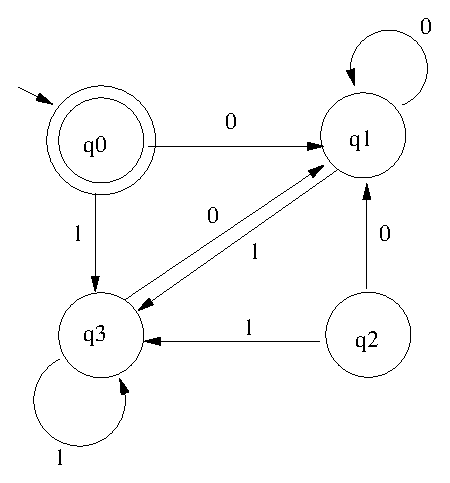
\includegraphics[width=8em]{fig}}
    \legend{Fonte: Os Autores}
    \label{fig:ex1}
\end{figure}

% o `[h]' abaixo é um parâmetro opcional que sugere que o LaTeX coloque a
% figura exatamente neste ponto do texto. Somente preocupe-se com esse tipo
% de formatação quando o texto estiver completamente pronto (uma frase a mais
% pode fazer o LaTeX mudar completamente de idéia sobre onde colocar as
% figuras e tabelas)
%\begin{figure}[h]
\begin{figure}
    \caption{Exemplo de figura desenhada com o environment \texttt{picture}.}
    \begin{center}
        \setlength{\unitlength}{.1em}
        \begin{picture}(100,100)
                \put(20,20){\circle{20}}
                \put(20,20){\small\makebox(0,0){a}}
                \put(80,80){\circle{20}}
                \put(80,80){\small\makebox(0,0){b}}
                \put(28,28){\vector(1,1){44}}
        \end{picture}
    \end{center}
    \legend{Fonte: Os Autores}
    \label{fig:ex2}
\end{figure}

Tabelas são construídas com praticamente os mesmos comandos. Ver a tabela \ref{tbl:ex1}.

\begin{table}[h]
    \caption{Uma tabela de Exemplo}
    \begin{center}
        \begin{tabular}{c|c|p{5cm}}
            \textit{Col 1}  &   \textit{Col 2}  &   \textit{Col 3} \\
            \hline
            \hline
            Val 1           &   Val 2           & Esta coluna funciona como um parágrafo, tendo uma margem definida em 5cm. Quebras de linha funcionam como em qualquer parágrafo do tex. \\
            Valor Longo     & Val 2             & Val 3 \\
            \hline
        \end{tabular}
    \end{center}
    \legend{Fonte: Os Autores}
    \label{tbl:ex1}
\end{table}

\subsection{Formato de Figuras}
\label{sec:fig_format}

O LaTeX permite utilizar vários formatos de figuras, entre eles \emph{eps}, \emph{pdf}, \emph{jpeg} e \emph{png}. Programas de diagramação como Inkscape (e mesmo LibreOffice) permitem gerar arquivos de imagens vetoriais que podem ser utilizados pelo LaTeX sem dificuldade. Pacotes externos permitem utilizar SVG e outros formatos.

Dia e xfig são programas utilizados por dinossauros para gerar figuras vetoriais. Se possível, evite-os.

\subsection{Classificação dos etc.}

O formato adotado pela ABNT prevê apenas três níveis (capítulo, seção e subseção). Assim, \texttt{\char'134subsubsection} não é aconselhado.

\section{Sobre as referências bibliográficas}

A classe \emph{iiufrgs} faz uso do pacote \emph{abnTeX2} com algumas alterações
feitas por Sandro Rama Fiorini. Culpe ele se algo der errado. Agradeça a ele
pelo que der certo. As modificações dão uma camada de tinta NATBIB-style,
já que o abntex2 usa uns comandos de citação feitos para alienígenas de 5 braços 
wtf. Exemplos de citação:

\begin{itemize}
    \item \emph{cite}: Unicórnios são verdes \cite{Adams2009Conceptual};
    \item \emph{citep}:Unicórnios são verdes \citep{Adams2009Conceptual};
    \item \emph{citet}: Segundo \citet{Adams2009Conceptual}, unicórnios são
                        verdes.
    \item \emph{citen or citenum}: Segundo \citen{Adams2009Conceptual},
        unicórnios são verdes.
    \item \emph{citeauthor e citeyearpar}: Segundo artigos de
        \citeauthor{Adams2009Conceptual} , unicórnios são verdes 
        \citeyearpar{Adams2009Conceptual}.

\end{itemize}

O estilo abnt fornecido antigamente pelo UTUG não é mais recomendado, pois não
produz saída de acordo com as exigências da biblioteca.

Recomenda-se o uso de bibtex para gerenciar as referências (veja o arquivo
biblio.bib).

% e aqui vai a parte principal
%
% \chapter{Estado da arte}
% \chapter{Mais estado da arte}
% \chapter{A minha contribuição}
% \chapter{Prova de que a minha contribuição é válida}
% \chapter{Conclusão}

% referencias
% aqui será usado o environment padrao `thebibliography'; porém, sugere-se
% seriamente o uso de BibTeX e do estilo abnt.bst (veja na página do
% UTUG)
%
% observe também o estilo meio estranho de alguns labels; isso é
% devido ao uso do pacote `natbib', que permite fazer citações de
% autores, ano, e diversas combinações desses

\bibliographystyle{abntex2-alf}
\bibliography{biblio}

\end{document}
